% 4.5 — Les filets d'exécution
\section{Les filets d'exécution}
\label{sec:filets}

\subsection{Linux : le garde d'appels système}
\fichier{syscall\_guard.py} lance la commande sous ptrace (\cmd{fork}, \cmd{PTRACE\_TRACEME},
puis \cmd{exec}) et suit aussi ses processus enfants (\cmd{fork}, \cmd{vfork}, \cmd{clone},
\cmd{exec}). À chaque arrêt sur appel système, il ne réagit qu'à l'\emph{entrée} de l'appel
(registre \cmd{rax} égal à \cmd{-ENOSYS}) et lit le numéro de l'appel et ses arguments dans
les registres x86-64 ; les chemins sont lus dans la mémoire du processus via
\cmd{/proc/<pid>/mem} et résolus par rapport au bon répertoire (\cmd{AT\_FDCWD} ou descripteur).

\begin{table}[htbp]
\centering
\caption{Appels système surveillés par le garde Linux}
\label{tab:syscalls}
\small
\begin{tabularx}{\linewidth}{@{}L{4.6cm}Y@{}}
\toprule
\textbf{Appel} & \textbf{Pourquoi il détruit} \\
\midrule
\cmd{unlink}, \cmd{unlinkat}, \cmd{rmdir} & suppression \\
\cmd{rename}, \cmd{renameat}, \cmd{renameat2} & la destination existante est remplacée \\
\cmd{creat}, \cmd{truncate} & le contenu est vidé \\
\cmd{open}, \cmd{openat} avec \cmd{O\_TRUNC} & le contenu est vidé à l'ouverture \\
\cmd{open}, \cmd{openat} en écriture sans \cmd{O\_APPEND} & réécriture en place \\
\bottomrule
\end{tabularx}
\end{table}

Pour un fichier préexistant du projet, la copie est prise, puis l'appel continue. Les fichiers
que la commande a elle-même créés ne sont pas copiés. Pour un fichier du plan de contrôle,
l'appel est annulé (le numéro d'appel est remplacé par $-1$) et un reçu ESCALATE est écrit. Si
le processus est déjà suivi par un traceur étranger (\cmd{strace}, \cmd{gdb}), le garde refuse
de s'exécuter sans surveillance (code de sortie 126). À la fin de la commande, les processus
d'arrière-plan sont détachés et continuent de tourner.

Voici le filet en action, sur le script réécrit par le \textit{hook} à la
section~\ref{sec:portes} ; le script supprime \cmd{notes.txt} et réécrit \cmd{src/app.py} :

\begin{terminal}[le filet capture au moment de la destruction]
$ demo_cli sh -g 8553dbf8 "python3 nettoyage.py"
demo_cli [syscall] REVERSIBLE: unlink ~/projet/notes.txt  (undo: demo_cli undo 8553dbf8)
demo_cli [syscall] REVERSIBLE: openat_trunc ~/projet/src/app.py  (undo: demo_cli undo 8553dbf8)
nettoyage terminé
\end{terminal}

Les deux fichiers ont été rendus par \cmd{demo\_cli undo 8553dbf8}
(section~\ref{sec:recuperation}). \demo{} n'a pas lu une ligne du script.

\subsection{Windows : le montage WinFsp}
Sous Windows, le filet est un système de fichiers. La mise en place (\cmd{demo\_cli setup},
\fichier{protect.py}) :
\begin{enumerate}
  \item déplace le projet \cmd{C:\textbackslash projet} vers \cmd{C:\textbackslash projet.real}
    (un point de montage WinFsp ne peut être créé que sur un répertoire vide ou absent ; un
    déplacement garde les chemins connus des outils et de l'IDE) ;
  \item verrouille \cmd{projet.real} par une ACL réservée aux Administrateurs et à SYSTEM ;
  \item monte à \cmd{C:\textbackslash projet} un système de fichiers « passe-plat » vers
    \cmd{projet.real}, exécuté avec élévation ;
  \item enregistre une tâche d'ouverture de session pour le remonter après un redémarrage.
\end{enumerate}
La figure~\ref{fig:cap-windows-setup} montre ces étapes sur un projet réel, puis leur exact
inverse : \cmd{demo\_cli teardown} arrête le montage, retire la tâche, remet les fichiers à leur
place et retire les \textit{hooks}, en laissant la configuration et les reçus comme trace d'audit.

\begin{figure}[htbp]
\centering
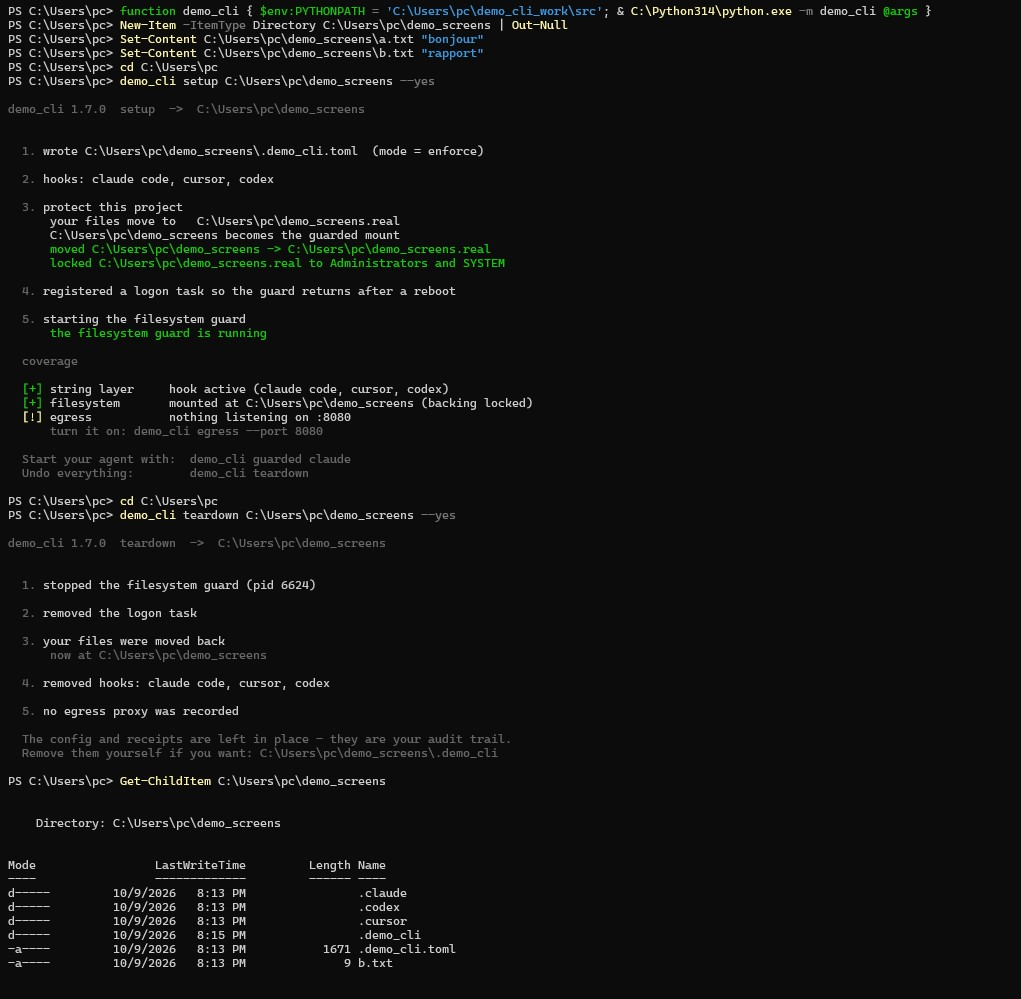
\includegraphics[width=0.95\linewidth]{figures/captures/windows-setup.png}
\caption{Sous Windows : \cmd{demo\_cli setup} protège un projet (déplacement, verrouillage, tâche,
montage), puis \cmd{demo\_cli teardown} défait chaque étape}
\label{fig:cap-windows-setup}
\end{figure}
Le montage a été construit en deux étapes qui prennent \emph{les mêmes décisions} : une
première version en mémoire, pour prouver l'interception, la capture et la restauration sans
risquer de corrompre de vrais fichiers ; puis la version passe-plat, sur laquelle on peut
travailler. Le passage de l'une à l'autre n'a demandé aucune modification du jugement
(\fichier{fsguard.py}) et une seule ligne de la capture : c'est le bénéfice d'avoir séparé le
jugement de la plomberie. Les captures sont écrites sur le disque réel, hors du montage.

\begin{figure}[htbp]
\centering
\capture{windows-montage}{Le montage actif (\cmd{doctor}) : un \cmd{Remove-Item} tapé dans le projet est capturé par le montage, qui ne lit aucune commande (entrée « delete a.txt » du journal de récupération)}%
{Sous Windows : \texttt{demo\_cli setup} sur un projet, puis l'Explorateur ou \texttt{Get-Item C:\textbackslash projet} montrant le point de montage, et \texttt{demo\_cli log} après un \texttt{Remove-Item} lancé par l'agent.}
\end{figure}

\subsection{Ce que les deux filets ne voient pas}
Les deux filets sauvegardent le projet, et seulement lui. Une destruction hors du projet par du
code non lu n'est pas sauvegardée ; le filet Linux l'\emph{enregistre} : un reçu par fichier,
sans sauvegarde ni blocage (V18, deuxième étape, \commitVdixhuit). Les répertoires
temporaires, \cmd{/proc}, \cmd{/sys}, \cmd{/dev}, les fichiers non réguliers et ceux que la
commande a créés elle-même sont ignorés, et une exécution est plafonnée à 100 reçus. La raison
de la décision le dit : « outside the project each destroyed file is recorded, not backed up ».
Le montage Windows ne voit que le projet.

\begin{terminal}[un script détruit un fichier dans le projet et un autre hors du projet]
$ demo_cli sh -g bbbb2222 "python3 nettoie.py"
demo_cli [syscall] REVERSIBLE: unlink ~/projet/notes.txt  (undo: demo_cli undo bbbb2222)
demo_cli [syscall] RECORDED (outside the project, not backed up): unlink ~/ailleurs/config.txt
fini
\end{terminal}

Le registre contient alors deux reçus : REVERSIBLE (\cmd{sys\_unlink}) avec un point de
récupération pour le fichier du projet, et ALLOW (\cmd{sys\_outside\_unlink}) sans point de
récupération pour le fichier extérieur --- « recorded, not backed up, cannot be undone ».

Les surfaces distantes leur sont invisibles : c'est pourquoi une ligne non lue
qui atteint le cloud, un conteneur ou un service escalade au lieu d'aller au filet.
